
\documentclass[conference]{IEEEtran}


% If IEEEtran.cls has not been installed into the LaTeX system files,
% manually specify the path to it like:
% \documentclass[conference]{../sty/IEEEtran}


% Some very useful LaTeX packages include:
% (uncomment the ones you want to load)


%\usepackage{fancyhdr}
\usepackage{cite}
%\usepackage{graphicx}
%\usepackage{psfrag}
%\usepackage{subfigure}
%\usepackage{url}
%\usepackage{stfloats}
%\usepackage{amsmath}
%\usepackage{array}
%\usepackage{fancyhdr}
%\usepackage{epsfig}
%\usepackage{amssymb}
%\usepackage{color}
\usepackage[T1]{fontenc}
\usepackage{mathtools} 
\usepackage{amsmath}
 \usepackage{graphicx}
\graphicspath{ {images/} }
\usepackage{subcaption}
\usepackage{subfig}
 % Some very useful LaTeX packages include:
% (uncomment the ones you want to load)
\usepackage{color}

\usepackage[letterpaper, left=1in, right=1in, bottom=1in, top=0.75in]{geometry}
% correct bad hyphenation here
\usepackage{algorithm,algorithmic}
\DeclarePairedDelimiter{\abs}{\lvert}{\rvert}
\DeclarePairedDelimiter{\norm}{\lVert}{\rVert}
\begin{document}
%
% paper title
% Titles are generally capitalized except for words such as a, an, and, as,
% at, but, by, for, in, nor, of, on, or, the, to and up, which are usually
% not capitalized unless they are the first or last word of the title.
% Linebreaks \\ can be used within to get better formatting as desired.
% Do not put math or special symbols in the title.
\title{A Smart Waste City Management System for Smart Cities Applications }


% author names and affiliations
% use a multiple column layout for up to three different
% affiliations


\author{\IEEEauthorblockN{Dung D. Vu}
\IEEEauthorblockA{Electrical Engineering Department\\
\'Ecole de Technologie Sup\'erieure\\
Email: do-dung.vu.1@ens.etsmtl.ca}
\and
\IEEEauthorblockN{Georges Kaddoum}
\IEEEauthorblockA{Electrical Engineering Department\\
	\'Ecole de Technologie Sup\'erieure\\
	Email:  georges.kaddoum@etsmtl.ca}}

% conference papers do not typically use \thanks and this command
% is locked out in conference mode. If really needed, such as for
% the acknowledgment of grants, issue a \IEEEoverridecommandlockouts
% after \documentclass

% for over three affiliations, or if they all won't fit within the width
% of the page, use this alternative format:
% 
%\author{\IEEEauthorblockN{Michael Shell\IEEEauthorrefmark{1},
%Homer Simpson\IEEEauthorrefmark{2},
%James Kirk\IEEEauthorrefmark{3}, 
%Montgomery Scott\IEEEauthorrefmark{3} and
%Eldon Tyrell\IEEEauthorrefmark{4}}
%\IEEEauthorblockA{\IEEEauthorrefmark{1}School of Electrical and Computer Engineering\\
%Georgia Institute of Technology,
%Atlanta, Georgia 30332--0250\\ Email: see http://www.michaelshell.org/contact.html}
%\IEEEauthorblockA{\IEEEauthorrefmark{2}Twentieth Century Fox, Springfield, USA\\
%Email: homer@thesimpsons.com}
%\IEEEauthorblockA{\IEEEauthorrefmark{3}Starfleet Academy, San Francisco, California 96678-2391\\
%Telephone: (800) 555--1212, Fax: (888) 555--1212}
%\IEEEauthorblockA{\IEEEauthorrefmark{4}Tyrell Inc., 123 Replicant Street, Los Angeles, California 90210--4321}}




% use for special paper notices
%\IEEEspecialpapernotice{(Invited Paper)}




% make the title area
\maketitle

% As a general rule, do not put math, special symbols or citations
% in the abstract
\begin{abstract}
This paper presents a new method of smart waste city management which makes the environment of the city cleanly with a low cost. In this approach, the sensor model detects, measures, and transmits waste volume data over the Internet. The collected data including trash bin's geolocation and the serial number is processed by using regression, classification, and graph theory. Thenceforth a new method is proposed to dynamically and efficiently manage the waste collection by predicting waste status, classifying trash bin location, and monitoring the amount of waste. Then, this latter recommends the optimization of the route to manage the garbage truck efficiently. Finally, the simulation results are presented and estimated
\end{abstract}

% no keywords




% For peer review papers, you can put extra information on the cover
% page as needed:
% \ifCLASSOPTIONpeerreview
% \begin{center} \bfseries EDICS Category: 3-BBND \end{center}
% \fi
%
% For peerreview papers, this IEEEtran command inserts a page break and
% creates the second title. It will be ignored for other modes.
\IEEEpeerreviewmaketitle



\section{Introduction}
\label{section1}
% no \IEEEPARstart
A smart city is an urban development vision to integrate information and communication technology (ICT) and Internet of things (IoT) technology which is the way of becoming the next technological revolution \cite{Delicato2013} securely to manage a city's assets. IoT is a framework in which all things have a representation and a presence on the Internet. More specifically, the IoT aims at offering new applications and services bridging the physical and virtual worlds, in which Machine-to-Machine (M2M) communication represents the baseline interface that enables the interactions between things and applications on the cloud such as environment monitoring \cite{Lazarescu2013}\cite{Kelly2013}, object tracking \cite{Gama2012}, traffic management \cite{Foschini2011}, health care \cite{Jara2011}, and smart home technology \cite{Tozlu2012}\cite{Li2011}. Organizations can use IoT to drive considerable cost savings by improving asset utilization, enhancing process efficiency and boosting productivity. IoT combines the exponential growth of smart devices,  the confluence of low-cost technologies (sensors, wireless networks, big data, and computing power), the pervasive connectivity, and the massive volumes of big data. Hence, IoT and big data are two sides of the same coin. An IoT device generates continuous streaming information in a scalable way. Companies must handle the high volume of stream data and perform actions on that one. These actions can be event correlation, matrix calculation, statistic preparation and analytic which are applied to construct the smart city. In the smart city, the waste management system is a crucial point of living environment, and its quality is considered seriously. A possible smart waste city management system requires a way to cluster the trash bin locations, detect the status of waste in each bin, and process this collected data. The result of this work will be a valuable input data for the garbage truck management system which calculates the most optimal route to prevent the hazard of damage, pollution of waste, and resource consumptions. 

\par To manage the waste of a smart city, the system incorporates a model for sharing data between truck drivers in the real time to perform garbage collection and the route optimization was proposed in \cite{Medvedev2015}. A waste collection solution based on providing intelligence of trash cans including sensors and IoT prototype, which can read, collect, and transmit trash volume data via wireless network was proposed in \cite{Gutierreza2015}\cite{Hong2014}. An adaptive large neighborhood search algorithm of finding optimal cost routes of garbage trucks was presented in \cite{Buhrkala212}, which processes the data of all emptied trash bins and the driven waste to disposal sites while respecting customer time windows. An improved dynamic route planning was discussed in \cite{Nuorito2006} where the authors enhanced a guided variable neighborhood threshold meta-heuristic adapted to the problem of waste collection. On the other hand, the most important part of a waste management system was the smart bin \cite{Sharma2015}\cite{Glouche2013}\cite{Sinhan2013} which collected the data of waste by using sensors and sent them over the internet to the server for monitoring the status of waste. While the network of ultrasonic sensors enabled smart bins to connect through the cellular network and generated a large amount of data which was further analyzed and visualized at real time to gain insights about the status of waste around the city \cite{Sharma2015}, a smart waste management with self-describing objects detected the kind of waste based on its Radio-frequency identification (RFID) information \cite{Glouche2013}. However, they did not know the hazard of each bin such as explosion or flame from the bottle of perfume, batteries, and electronic wastes. In \cite{Sinhan2013}, a hazard detection method was proposed to detect and prevent these issues. Hence, a waste city management was conducted by an optimal garbage truck routes algorithm based on the status of the smart bin. 

However, we observed that citizens in the city tend to throw their waste into the trash bins without a particular time of a day and the manager needs to add more bins during the holiday event time. As previous works do not solve this issue, the novelty of our work proposes a new method to automatically classify the location of trash bins, predict the status of each one, and optimize the garbage truck routes. The aim of this proposition is to help the city’s waste management system to operate more efficiently. 

\par\textbf{Contributions:} 
This paper presents a new method of smart waste city management which provides a clean and hygienic environment to the city resident. In this approach, the collected data from the trash bin has been transferred over the Internet to the server which contains the status of each bin. The contributions of this paper are summarized as follows:

\begin{figure}
	\centering
	\parbox{5cm}{
		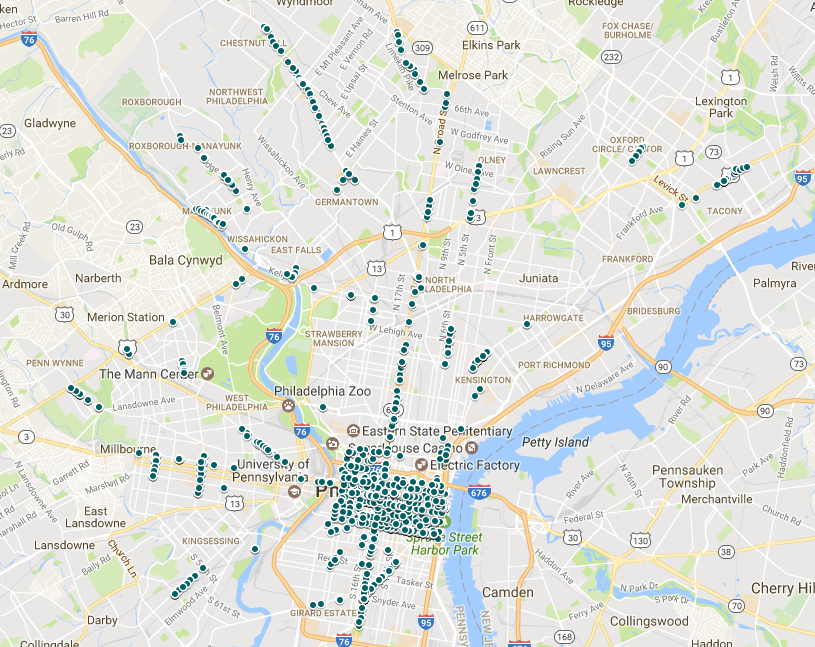
\includegraphics[width=5cm]{overview1}
		\subcaption{The whole distribution of trash bin}
		\label{fig1a}}
	\qquad
	\begin{minipage}{5cm}
		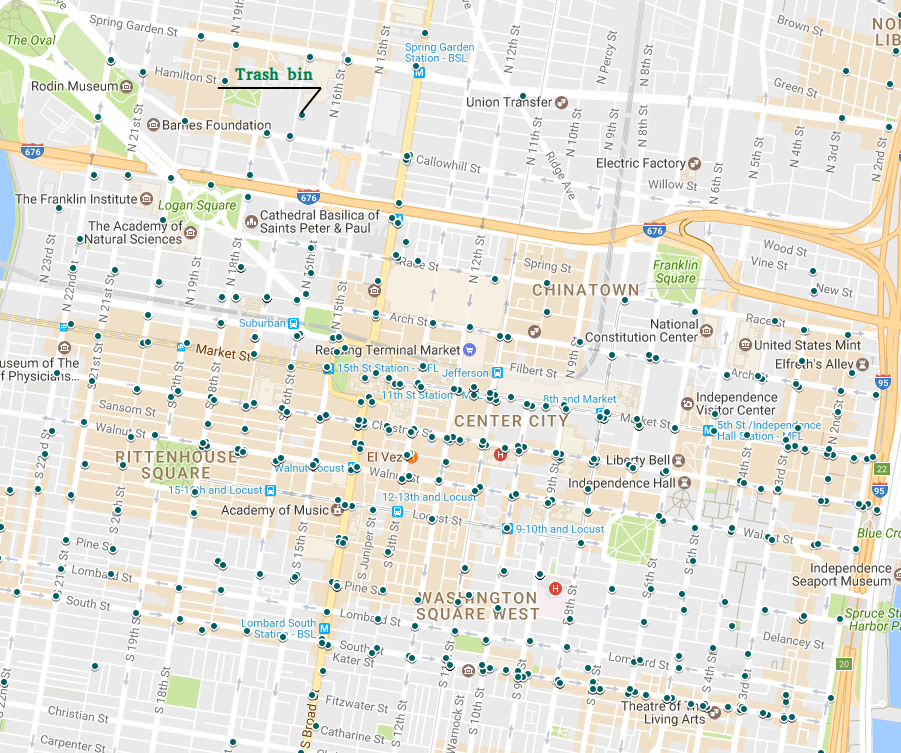
\includegraphics[width=5cm]{overview3}
		\subcaption{A part of distribution trash bin}
		\label{fig1b}
	\end{minipage}
	\caption{Philadelphia trash bin}
	\label{Philadelphia}
\end{figure}

\begin{itemize}
	\item The number of working clusters in each city are optimized and the location of new trash bins are classified automatically. 
	
	\item A regression algorithm is applied to predict the situation of waste which can reduce the overload trash bin phenomenon while the garbage truck is coming.
	
	\item The priority weight of each bin is considered to improve the optimal garbage truck routes algorithm more efficiently.
	
\end{itemize}

Finally, to the best of authors’ knowledge, no result exists before our contribution. 

This paper is organized as the follows: In section \ref{section2},  a new method of smart waste city management (SWCM) is explained and the structure of the algorithm is proposed. Section \ref{section3} presents the SWCM simulation model. Finally, the related concluding remarks are discussed in section \ref{section4}.



\section{IoT-Based Smart waste management model}
\label{section2}
In this section, we describe how to collect waste metadata associated with their statuses and locations. We evaluate our model with real big data in order to validate its output result.
\subsection{Data acquisition} 


\par To obtain a set of waste data, we use an open source database,\footnote{https://www.opendataphilly.org/dataset} which has a significant amount of geo-location information and status of trash bins at the largest city in the Commonwealth of Pennsylvania in the United Stated named Philadelphia. Figure \ref{Philadelphia} illustrates the distribution of trash bin (green node) in Philadelphia city. Since there are many contents in this data, we removed the content that was not related to our scenario. For data analysis, five essential fields from this metadata are presented in the Table \ref{t1}.

\begin{table}[]
	\centering
	\caption{The trash bin dataset}
	\label{t1}
	\begin{tabular}{|l|l|}
		\hline
		\multicolumn{1}{|c|}{Field} & 	\multicolumn{1}{|c|}{Description} \\ \hline
		\textit{sn} &  The serial number of each trash bin\\ \hline
		\textit{time\_stamp} &  The milestone of recording data\\ \hline
	\textit{level} &  \begin{tabular}[c]{@{}l@{}}The amount of waste in each trash bin\\ (GREEN, YELLOW, RED) at the given time \end{tabular} \\ \hline
	\textit{lat} &  The latitude of each trash bin\\ \hline
	\textit{lon} &  The longitude of each trash bin\\ \hline
	\end{tabular}
\end{table}




\subsection{System description}
\label{systemdesciption}
\subsubsection{The overview of functionality}


The proposed system is based on the waste status of each trash bin in the city. The collected data is sent over the Internet to the server where it is stored and processed. At here, it is used for monitoring and predicting the status of each trash bin daily. Moreover, it will be utilized for calculating the optimal garbage truck routes, accordingly. The prediction status of each bin can be analyzed based on the given training data before it occurs. Then, it will be considered to update the weight of the trash bin accordingly which is the most important input parameter of optimal garbage truck routes algorithm. The system overview is shown in the Figure \ref{fig2}.


\subsubsection{Data processing and classifications}


The status of each bin is not homogeneous and significantly differs from each other according to the state of each location. In this section, we introduce an algorithm that can be used to dynamically and efficiently manage waste collection strategies.
\begin{figure}
	\centering
	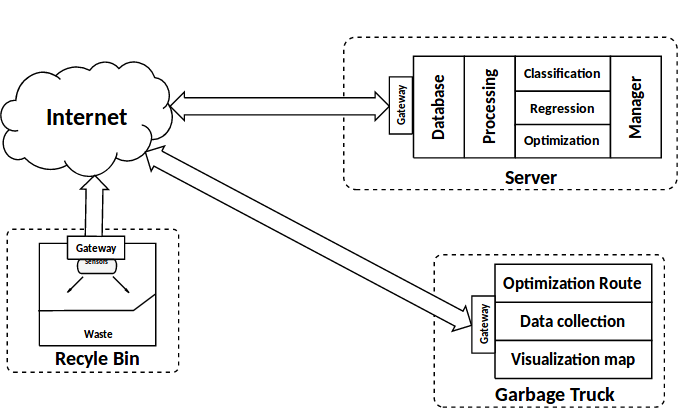
\includegraphics[width=7.5cm]{Model1-2}
	\caption{The smart waste management system overview}
	\label{fig2}
\end{figure}

\par K-means \cite{Kanungo2003} is an unsupervised machine learning algorithm that groups a dataset into a user-specified number ($k$) of clusters. We use it to make the working cluster of each garbage truck. However, this algorithm is somewhat naive, it clusters the data into $k$ clusters, even if $k$ is not the right number of clusters to use. Therefore, when using k-means clustering, users need some way to determine whether they are using the right number of clusters. In this paper, we use Elbow method \cite{Kodinariya2013} \cite{Maria2001} to validate the number of clusters. The collecting routes are the traveling cycles containing a set of trash bins within a given cluster. The optimization of these cycles is a combinatorial optimization problem. By considering a large number of routes, we use a Genetic Algorithm (GA) \cite{Gutierrez2008} which are relatively fast in providing near optimal solutions. Since the garbage truck needs time to collect every trash bin, it is very delightful if a status of trash bin can be predicted. Hence, after predicting, the system will recommend which one should be collected to prevent the overload phenomenon. In this paper, we use the Logistic regression algorithm \footnote{https://nlp.stanford.edu/manning/courses/ling289/logistic.pdf} to predict the status of each trash bin based on its historical data.


\par  The overall procedure is summarized in Algorithm \ref{algorithm1}. In this algorithm, the parameters are defined in Table \ref{table1}. We suppose that the input dataset $\mathcal{D}$ is the database in Section \ref{section2}. At the given time stamp $t$, a logistic regression (LR) algorithm is applied to predict the status of each bin. If the prediction status $s_{jh}$ of bin is greater than the given threshold $\eta$, the weight $w_{jh}$ is updated to $1$, respectively, then the GA algorithm is utilized to minimize the driving distance for visiting the selected bins and returning to the headquarters. Therefore, we find the optimal garbage truck routes in each cluster $M_j$ which help us to prevent the collect trash bin more efficiently.
\begin{table}[]
	\centering
	\caption{The definition of each variable}
	\label{table1}
	\begin{tabular}{|l|l|}
		\hline
	
				\multicolumn{1}{|c|}{Variable} & \multicolumn{1}{|c|}{Description} \\ \hline
		$S=\{s_{i} | i \in (1,n) \}$	& \begin{tabular}[c]{@{}l@{}}The status of each bin   $i$   \end{tabular}       \\ \hline
		$L=\{l_{i} | i \in (1,n) \}$	& \begin{tabular}[c]{@{}l@{}}The location of each bin   $i$   \end{tabular}       \\ \hline
		$W=\{w_i | i \in (1,n)\}$	& The weight of each bin $i$            \\ \hline
		$T=\{t_{di} | d \in (1,m); i \in (1,n) \}$	& \begin{tabular}[c]{@{}l@{}}The collected data milestone \\of each bin     $i$ \end{tabular}       \\ \hline
		
		$\mathcal{D}=\{S,L,W, T\}$	& The input data         \\ \hline

		
		$\mathcal{M}=\{M_j | j \in (1,k)\}$	& 
		
		\begin{tabular}[c]{@{}l@{}}The optimal route of each garbage \\truck within each cluster $M_j$\end{tabular}
		\\ \hline
		\begin{tabular}[c]{@{}l@{}}
			$\mathcal{DC}=\{DC_j | j \in (1,k)$; \\$DC_j = \{S_j, L_j, W_j, T_j\} \}$	\end{tabular}& 
		
		\begin{tabular}[c]{@{}l@{}}The working cluster\end{tabular}
		\\ \hline
		
		$k$	& The number of working clusters         \\ \hline
		
				$\eta$	& The threshold of amount waste       \\ \hline
		
					$n$	& \begin{tabular}[c]{@{}l@{}}The number of trash bins in the \\dataset \end{tabular}    \\ \hline
		
				$m()$	& \begin{tabular}[c]{@{}l@{}}The dynamic vector of number\\ trash bins in each working cluster\end{tabular}    \\ \hline
				
		
	\end{tabular}
	
\end{table}





\section{Analysis result and discussion}
\label{section3}
\begin{algorithm}[]
	\caption{}
	\begin{algorithmic}[1]
		\renewcommand{\algorithmicrequire}{\textbf{Input:}}
		\renewcommand{\algorithmicensure}{\textbf{Output:}}
		\REQUIRE $\mathcal{D}, \eta$
		\ENSURE  $\mathcal{M}$
		\\ \textit{Initialization}: $j, k, h, m() = 0, k = [1;15]$
		\STATE $k^*$ = Elbow($\mathcal{D}\rightarrow$L, $n$)
		\STATE $\mathcal{DC}$ = K-means($\mathcal{D}\rightarrow$L, $k^*$)
	

		\STATE At a given time stamp $t$ in the near future.
		\FOR {$j = 1$ to $k^*$}
			\STATE $m_j$ = size($\mathcal{DC}_j$)
		\FOR {$h = 1$ to $m_j$}
		
		\STATE $s_{jh}$ = LR($DC_j \rightarrow S_j, DC_j \rightarrow T_j$)
		\IF {($s_{jh} \ge \eta$)}
		\STATE $w_{jh} = 1$
		\STATE $M_j$ = GA($DC_j \rightarrow L_j, DC_j \rightarrow W_j$)
		\ENDIF
		
		\ENDFOR
		\STATE Plot ($M_j$)
		\ENDFOR
		
	\end{algorithmic} 
	\label{algorithm1}
\end{algorithm}

In this section, using the proposed Algorithm \ref{algorithm1} in Section \ref{systemdesciption}, we first analyze the number of working cluster and then show the experimental result. We simply assume $\eta = 0.5$, which can also to be set another value to monitor the amount of waste. 

\subsection{Number of working cluster}

\begin{figure}
	\centering
	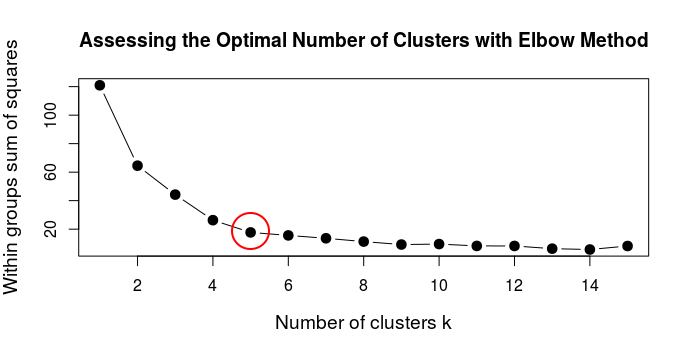
\includegraphics[width=6cm]{elbow6}
	\caption{The optimal value of number working clusters}
	\label{fig3}
\end{figure}



One  method of validating the number clusters for K-means algorithm is the Elbow method. It looks at the percentage of variance explained as a function of the number of clusters: One should choose a number of clusters so that adding another cluster does not give much better modeling of the data. In the general, $k \in [1;\infty]$ but for the simple experiment, we choose $k\in[1;15]$ in our work. To estimate the optimal value of $k^*$, we use the function Elbow($\mathcal{D}\rightarrow$L, $n$) which considers the value within-cluster variance $W(DC_j)$ of a cluster $DC_j$ which is defined as $\sum_{l_i\in DC_j}\norm{l_i-\bar{l_j}}^2$, where $\bar{l_j}$ is the mean of cluster $DC_j$ (also called the cluster centroid, its values are the coordinate-wise average fo the data points in $DC_j$), and $\{l_1, l_2,..., l_n\}$ is the set of trash bin location. The total within cluster scatter is $W = \sum_{j=1}^{k}\sum_{l_i\in DC_j}\norm{l_i-\bar{l_j}}^2$ for $k$ clusters and $n$ observations. A good choice value of $k^*$ is considered if this value tends to change slowly and remain less changing as compared to other $k$'s.\footnote{https://www.r-bloggers.com/finding-optimal-number-of-clusters/} We see a pretty clear Elbow at $k^* = 5$ in Figure \ref{fig3} and table \ref{tab3}, which indicates that $5$ is the best number of clusters.




\par Using the value of $k^*$ above, we apply the K-means algorithm to make the working clusers for our system. The output is represented in the Figure \ref{fig4}. If the manager tend to add more trash bins into our system, the system will automatically update these working clusters.

\begin{figure}
	\centering
	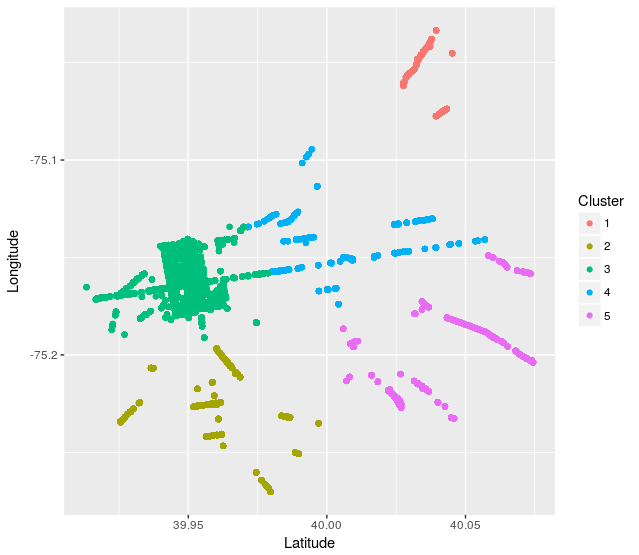
\includegraphics[width=6.5cm]{workingcluster}
	\caption{The working clusters in Philadelphia}
	\label{fig4}
\end{figure}
\begin{table}[]
	\centering
	\caption{The value output of Elbow function}
	\label{tab3}
	\begin{tabular}{|l|l|l|l|}
		\hline
		\multicolumn{1}{|c|}{$k$} &\begin{tabular}[c]{@{}l@{}} Total within cluster sum of square WSS\end{tabular} & \multicolumn{1}{|c|}{Gap}  \\ \hline
		1	& 120.955074  &  56.4187142 \\\hline
		2	&  64.536360  &  22.1861431 \\ \hline
		3	& 42.350217  &   16.7424861 \\ \hline
		4	& 25.607731  &    7.8911692 \\\hline
		5	& 17.716561  &   2.9992944 \\ \hline
		6	& 14.717267  &  2.3197915 \\ \hline
		7	& 12.397475  &   1.8433894 \\\hline
		8	& 10.75307  &    1.6211788 \\ \hline
		9	& 8.932907   &   1.5458681 \\ \hline
		10	&  7.387039   &   0.7622440  \\ \hline
		11	& 6.848576   &0.5217154   \\ \hline
		12	&  6.130773   &  0.5949759 \\ \hline	13	& 5.775266  &  0.2314699 \\ \hline
		
		14	& 5.346625 & 0.5413839  \\ \hline
		15	& 4.894336  &   NA\\ \hline
	\end{tabular}
\end{table}

\subsection{Prediction the status of trash bin} 

In fact, when the garbage trucks are running on the road, the status of trash bins can be modified. It is very delightful to predict the status of trash bin, then update the weight of this one. After that, the system will update the optimal garbage truck route. A Logistic regression algorithm is applied to work on this issue. 

We pick up randomly one trash bin in one cluster whose serial number and location are $171758$ and ($39.95204^o,-75.15911^o$), respectively to analyze the output result for convenience. Fistly, We convert all the date to the numeric data type\footnote{https://cran.r-project.org/web/packages/lubridate/lubridate.pdf} which is utilized for the Logistic regression algorithm. Figure \ref{fig5a} represents the relation between weight (green circle) and the time stamp of this trash bin. In this figure, the red line represents the trend of trash bin's weight. By considering a given time, if the red line approaches the value $1$, the weight of trash bin will be updated to $1$, respectively. Hence, the optimal garbage truck route will be constructed based on the new weight.
\begin{figure}
	\centering

	\begin{minipage}{5cm}
	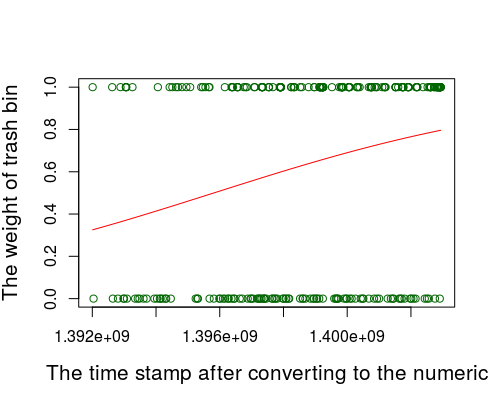
\includegraphics[width=5cm]{regression}
	\subcaption{The LR of the $171758^{th}$ trash bin}
	\label{fig5a}
\end{minipage}
	\begin{minipage}{5cm}
	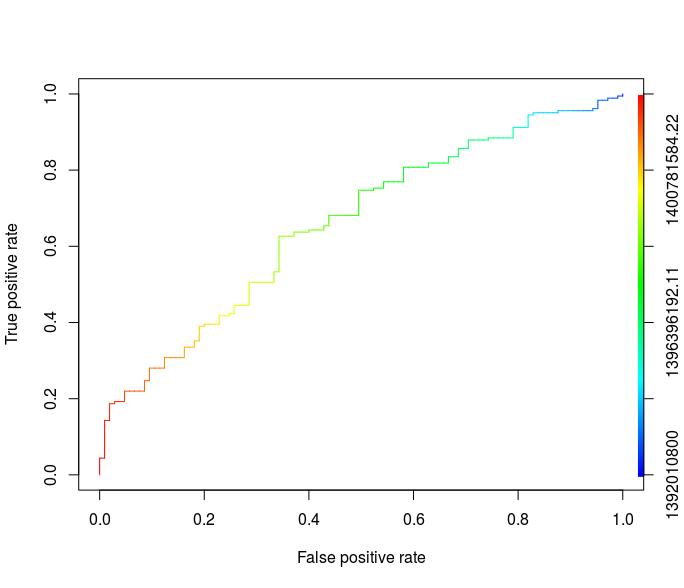
\includegraphics[width=5cm]{roc}
	\subcaption{The ROC curve of the output LR of the $171758^{th}$ trash bin  }
	\label{fig5b}
\end{minipage}
\label{fig5}
	\caption{The logistic regression result of the $171758^{th}$ trash bin}
\end{figure}

\subsection{Optimal route of garbage truck in each cluster}

\begin{figure}
	\centering
	\begin{minipage}{3.5cm}
		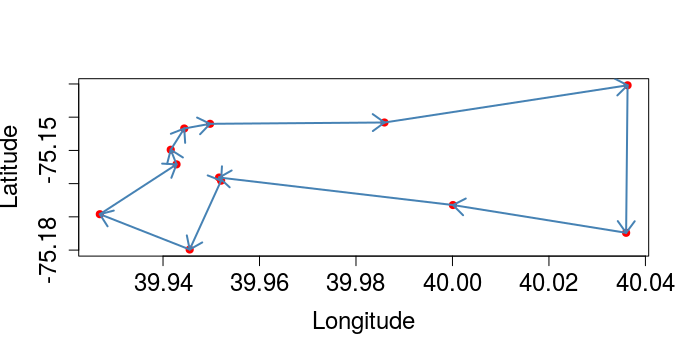
\includegraphics[width=3.5cm]{Cluster1}
		\subcaption{Cluster 1}
		\label{fig1a}
			\end{minipage}
	\begin{minipage}{3.5cm}
		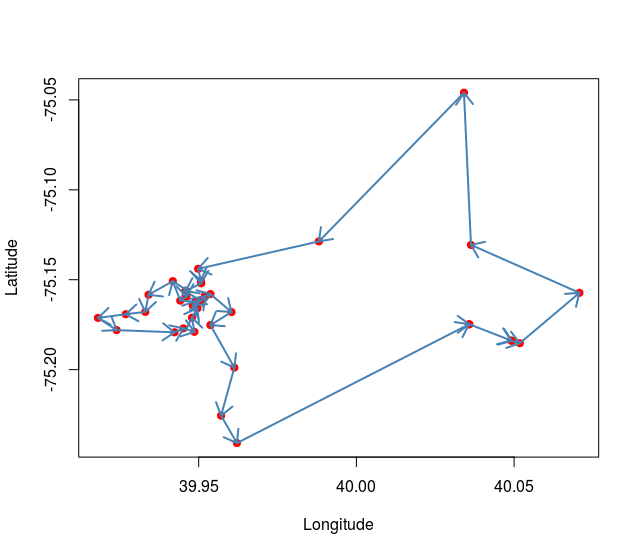
\includegraphics[width=3.5cm]{Cluster2}
		\subcaption{Cluster 2}
		\label{fig1b}
	\end{minipage}
	
	
		\begin{minipage}{3.5cm}
		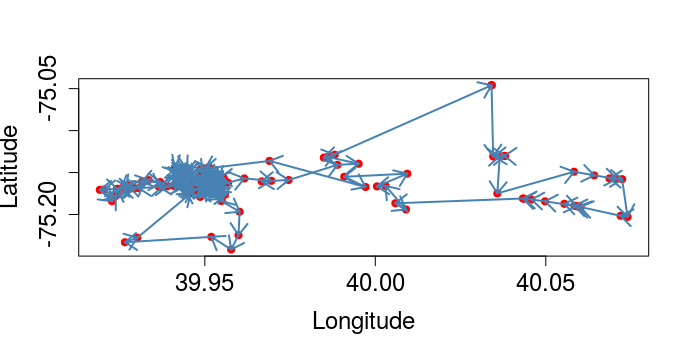
\includegraphics[width=3.5cm]{Cluster3}
		\subcaption{Cluster 3}
		\label{fig1a}
			\end{minipage}
	\begin{minipage}{3.5cm}
		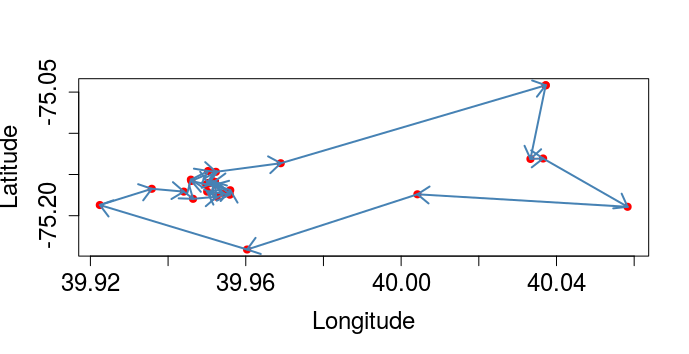
\includegraphics[width=3.5cm]{Cluster4}
		\subcaption{Cluster 4}
		\label{fig1b}
	\end{minipage}
	
	
	\begin{minipage}{5cm}
		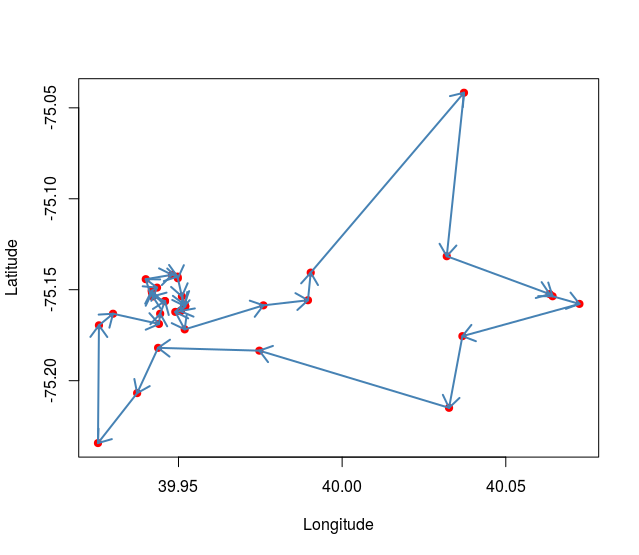
\includegraphics[width=3.5cm]{Cluster5}
				\subcaption{Cluster 3.5}
		\label{fig1b}
	\end{minipage}
	\caption{The optimal route of garbage truck at 2014-06-16}
	\label{fig5}
	
\end{figure}

In the each cluster dataset $\mathcal{DC}_j$, where $j \in [1:k]$, we observed that the original system has three status levels of bin such as RED, YELLOW, and GREEN. Let we assume that when $\eta = 0.5$ the trash bin's level is RED or YELLOW and its weight is $1$, otherwise it is $0$.

\par Since we need to update the optimal garbage truck routes daily for collecting the high weight trash bin, so we would like to pick up a milestone randomly which is ``2014-06-16" in our dataset to make the simulation. By using the GA algorithm, the optimal garbage truck routes of each working cluster are constructed based on the weight and coordinate of trash bins. In the Figure \ref{fig5}, the red point is the high weight trash bin and the arrow is the route of garbage truck. It means that the garbage trucks collected all the trash bin whose weigh is $1$ by using the optimal routes. Hence, the system will help the smart city to reduce the traffic congestion, fuel consumption, and pollution.






\section{Conclusion and future works}
\label{section4}

In this paper, we first clustered the working area by using the open source database of Philadelphia. Especially, we introduced an algorithm which automatically makes the working clusters and calculates the optimal garbage truck routes. Also, we use the Logistic regression to predict and update the weight of each trash bin. They will be used for creating the new optimal garbage route which reduces the pollution and fuel consumption more efficiently.  

To further improve the algorithm, future work, the optimal garbage truck routes within each cluster need to be fitted with the street map data.


% An example of a floating figure using the graphicx package.
% Note that \label must occur AFTER (or within) \caption.
% For figures, \caption should occur after the \includegraphics.
% Note that IEEEtran v1.7 and later has special internal code that
% is designed to preserve the operation of \label within \caption
% even when the captionsoff option is in effect. However, because
% of issues like this, it may be the safest practice to put all your
% \label just after \caption rather than within \caption{}.
%
% Reminder: the "draftcls" or "draftclsnofoot", not "draft", class
% option should be used if it is desired that the figures are to be
% displayed while in draft mode.
%
%\begin{figure}[!t]
%\centering
%\includegraphics[width=2.5in]{myfigure}
% where an .eps filename suffix will be assumed under latex, 
% and a .pdf suffix will be assumed for pdflatex; or what has been declared
% via \DeclareGraphicsExtensions.
%\caption{Simulation results for the network.}
%\label{fig_sim}
%\end{figure}

% Note that the IEEE typically puts floats only at the top, even when this
% results in a large percentage of a column being occupied by floats.


% An example of a double column floating figure using two subfigures.
% (The subfig.sty package must be loaded for this to work.)
% The subfigure \label commands are set within each subfloat command,
% and the \label for the overall figure must come after \caption.
% \hfil is used as a separator to get equal spacing.
% Watch out that the combined width of all the subfigures on a 
% line do not exceed the text width or a line break will occur.
%
%\begin{figure*}[!t]
%\centering
%\subfloat[Case I]{\includegraphics[width=2.5in]{box}%
%\label{fig_first_case}}
%\hfil
%\subfloat[Case II]{\includegraphics[width=2.5in]{box}%
%\label{fig_second_case}}
%\caption{Simulation results for the network.}
%\label{fig_sim}
%\end{figure*}
%
% Note that often IEEE papers with subfigures do not employ subfigure
% captions (using the optional argument to \subfloat[]), but instead will
% reference/describe all of them (a), (b), etc., within the main caption.
% Be aware that for subfig.sty to generate the (a), (b), etc., subfigure
% labels, the optional argument to \subfloat must be present. If a
% subcaption is not desired, just leave its contents blank,
% e.g., \subfloat[].


% An example of a floating table. Note that, for IEEE style tables, the
% \caption command should come BEFORE the table and, given that table
% captions serve much like titles, are usually capitalized except for words
% such as a, an, and, as, at, but, by, for, in, nor, of, on, or, the, to
% and up, which are usually not capitalized unless they are the first or
% last word of the caption. Table text will default to \footnotesize as
% the IEEE normally uses this smaller font for tables.
% The \label must come after \caption as always.
%
%\begin{table}[!t]
%% increase table row spacing, adjust to taste
%\renewcommand{\arraystretch}{1.3}
% if using array.sty, it might be a good idea to tweak the value of
% \extrarowheight as needed to properly center the text within the cells
%\caption{An Example of a Table}
%\label{table_example}
%\centering
%% Some packages, such as MDW tools, offer better commands for making tables
%% than the plain LaTeX2e tabular which is used here.
%\begin{tabular}{|c||c|}
%\hline
%One & Two\\
%\hline
%Three & Four\\
%\hline
%\end{tabular}
%\end{table}


% Note that the IEEE does not put floats in the very first column
% - or typically anywhere on the first page for that matter. Also,
% in-text middle ("here") positioning is typically not used, but it
% is allowed and encouraged for Computer Society conferences (but
% not Computer Society journals). Most IEEE journals/conferences use
% top floats exclusively. 
% Note that, LaTeX2e, unlike IEEE journals/conferences, places
% footnotes above bottom floats. This can be corrected via the
% \fnbelowfloat command of the stfloats package.







% conference papers do not normally have an appendix


% use section* for acknowledgment







% trigger a \newpage just before the given reference
% number - used to balance the columns on the last page
% adjust value as needed - may need to be readjusted if
% the document is modified later
%\IEEEtriggeratref{8}
% The "triggered" command can be changed if desired:
%\IEEEtriggercmd{\enlargethispage{-5in}}

% references section

% can use a bibliography generated by BibTeX as a .bbl file
% BibTeX documentation can be easily obtained at:
% http://mirror.ctan.org/biblio/bibtex/contrib/doc/
% The IEEEtran BibTeX style support page is at:
% http://www.michaelshell.org/tex/ieeetran/bibtex/
%\bibliographystyle{IEEEtran}
% argument is your BibTeX string definitions and bibliography database(s)
%\bibliography{IEEEabrv,../bib/paper}
%
% <OR> manually copy in the resultant .bbl file
% set second argument of \begin to the number of references
% (used to reserve space for the reference number labels box)
\begin{thebibliography}{1}


\bibitem{Delicato2013}
F. C. Delicato, P. F. Pires,  T. Batista, E. Cavalcante, B. Costa, and  T. Barros, \emph{Towards an IoT eco-system}, In the Proceedings of the 1st ACM International Workshop on Software Engineering for Systems-of-Systems, SESoS’13, 2013, pp. 25--28.


\bibitem{Lazarescu2013}
M. T. Lazarescu, \emph{Design of a WSN platform for long-term environmental monitoring for IoT application}, IEEE Journal on Emerging and Selected Topics in Circuits and Systems, Volume 3, Number 1 (2013): 45--54.



\bibitem{Kelly2013}
S. D. T. Kelly, N. K. Suryadevara, and S. C. Mukhopadhyay, \emph{Towards the implementation of IoT for environmental condition monitoring in homes}, IEEE Sensors Journal, Volume 13, Number 10 (2013): 3846--3853.

\bibitem{Gama2012}
K. Gama, L. Touseau, and D. Donsez, \emph{Combining heterogeneous service technologies for building an internet of things middle-ware}, Computer Communications, Volume 35, Number 4 (2012): 405--417.


\bibitem{Foschini2011}
L. Foschini, T, Taleb, A. Corradi, and D. Bottazzi, \emph{M2M-based metropolitan platform for IMS-enabled road traffic management in IoT}, IEEE Communications Magazine, Volume 49, Number 11 (2011): 50--57.


\bibitem{Jara2011}
A. J. Jara, A. Zamora, and A. F. G. Skarmeta, \emph{An internet of things-based personal device for diabetes therapy management in ambient assited living (AAL)}, Personal and Ubiquitous Computing, Volume 15, Number 4 (2011): 431--440.




\bibitem{Tozlu2012}
S. Tozlu, M. Senel, W. Mao, and A. Keshavarzian, \emph{Wi-Fi enabled sensors for internet of things: A pratical approach}, IEEE Communications Magazine, Volume 50, Number 6 (2012): 134--143.

\bibitem{Li2011}
X. Li, R. Lu, X. Liang, X. Shen, J. Chen, and X. Lin, \emph{Smart community: An internet of things appilication}, IEEE Communications Magazine, Volume 49, Number 11 (2011): 68--75.

\bibitem{Medvedev2015}
A. Medvedev, P. Fedchenkov, A. Zaslavsky, T. Anagnostopoulos, and S. Khoruzhnikov, \emph{Waste management as an IoT enabled service in smart cites}, 15th ed, St. Petersburg, Russia: Internet of Things, Smart Spaces, and Next Generation Networks and Systems, 2015, pp 104--115.



\bibitem{Gutierreza2015}
J. M. Gutierreza, M. Jensenb, M. Heniusa, and T. Riaze, \emph{Smart waste collection system based on location intelligence}, Procedia Computer Science 61 (2015): 120--127.


\bibitem{Hong2014}
J. Hong, S. Park, B. Lee, J. Lee, D. Jeong, and S. Park, \emph{IoT-based smart garbage system for efficient food waste management}, The Scientific World Journal (2014).




\bibitem{Buhrkala212}
K. Buhrkala, A. Larsena, and S. Ropkea, \emph{The waste collection vehicle routing problem with time windows in a city logistics context}, Procedia Social and Behavioral Sciences 39 (2012): 241--254.


\bibitem{Nuorito2006}
T. Nuortio, J. Kyt\"ojoki, H. Niska, and O. Br\"aysy, \emph{Improved route planning and scheduling of waste collection and transport}, Expert Systems with Applications, Volume 30, Issue 2 (2006): 223--232.


\bibitem{Sharma2015}
N. Sharma, N. Singha, and T. Dutta, \emph{Smart bin implementation for smart cities}, International Journal of Scientific \& Engineering Research (2015), Volume 6, Issue 9: 787--791.


\bibitem{Glouche2013}
Y. Glouche and P. Couderc, \emph{A smart waste management with self-describing objects}, The second International Conference on Smart Systems, Devices, and Technologies, 2013, pp 63--70.


\bibitem{Sinhan2013}
A. Sinhan and P. Couderc, \emph{Smart bin for imcompatible waste items}, The ninth International Conference on Autonomic and Autonomous Systems, 2013, pp 40--45.


\bibitem{Kanungo2003}
T. Kanungo, D.M. Mount, N.S. Netanyahu, C.D. Piatko, R. Silverman, and A.Y. Wu, \emph{An efficient k-means clustering algorithm: Analysis and implementation}, IEEE Transactions on Pattern Analysis and Machine Intelligence, Volume 24, Issue 7 (2002): 881--892.


\bibitem{Kodinariya2013}
T. M. Kodinariya and P. R. Makwana, \emph{Review on determining number of cluster in K-means clustering}, International Journal of Advance Research in
Computer Science and Management Studies, Volume 1, Issue 6 (2013): 90--95.

\bibitem{Maria2001}
M. Halkidi, Y. Batistakis, and M. Vazirgiannis, \emph{On clustering validation techniques}, Journal of Intelligent Information System, 17:2/3 (2001): 107 -- 145.

\bibitem{Gutierrez2008}
J. M. Gutierrez, M. Imine, and O. B. Madsen, \emph{Network planning using GA for regular topologies}, Proceedings of IEEE International Conference on Communications, 2008, pp: 5258--5262.


\end{thebibliography}




% that's all folks
\end{document}


